% ============================================================
%  Supplement: linear algebra in GNSS
%
%  Study material for readers who come to the estimator from an
%  advanced linear algebra course: vector and matrix norms,
%  Hermitian matrices, the SVD and the pseudoinverse, each tied to a
%  computation in this engine through thirteen numerical examples.
%  Every number is printed by scripts/linalg_supplement_examples.py
%  (numpy only, one seed per example).  Where the engine's own
%  version of a result is derived in another component, the text
%  links to it with \dcref instead of repeating it.
%
%  Standalone-compilable subfile (shares gnssreport.sty via the
%  subfiles package).  Wired into the combined volume as an appendix
%  after \subfile{generated_tables} in main.tex.
% ============================================================
\documentclass[main.tex]{subfiles}
\begin{document}
\ifSubfilesClassLoaded{\begin{center}\small\itshape Part of the GnssProcessor Mathematical Reference \textbullet\ \today\end{center}}{}

\section{Supplement: linear algebra in GNSS}\label{sec:linalg}

This supplement connects four topics of an advanced linear algebra course to
computations that recur in GNSS positioning: vector and matrix norms,
Hermitian matrices (real symmetric, in estimation), the singular value
decomposition (SVD), and the Moore--Penrose pseudoinverse.  Thirteen
numerical examples carry the argument.  All of them use one simulated epoch
(\Cref{sec:la-model}), and every number is printed by
\texttt{scripts/linalg\_supplement\_examples.py} (\Cref{sec:la-reproduce}).
Where the engine's own version of a result is derived elsewhere in this
reference, the text links to it.

\subsection{The model used throughout}\label{sec:la-model}

Linearised GNSS observation equations have the form
\begin{equation}
\bm{y} = \bm{A}\,\bm{x} + \bm{\varepsilon},
\qquad
\mathsf{E}\{\bm{\varepsilon}\} = \bm{0},
\qquad
\mathsf{D}\{\bm{\varepsilon}\} = \Rmat,
\label{eq:la-gmm}
\end{equation}
with $m$ observations, $n$ parameters and observation covariance $\Rmat$.
For code positioning the design matrix is the geometry matrix $\bm{G}$, with
one row per satellite,
\begin{equation}
\bm{g}_\sat^\Tr = \begin{bmatrix} -\los_\sat^\Tr & 1 \end{bmatrix},
\label{eq:la-grow}
\end{equation}
where $\los_\sat$ is the unit line of sight to satellite $\sat$, expressed
here in local east, north and up components, and the last column belongs to
the receiver clock $\sLight\,\mathrm{d}t_\rx$, kept in metres
(\dcref{eq:geom-linear}{the linearised geometric range of the Foundations
document}).  One epoch of code and phase on a single frequency adds one
float ambiguity $N_\sat$, in cycles, per satellite:
\begin{equation}
\code_\sat = \bm{g}_\sat^\Tr\bm{x} + \varepsilon^\code_\sat,
\qquad
\phaseo_\sat = \bm{g}_\sat^\Tr\bm{x} + \lambda_{\mathrm{L1}} N_\sat
               + \varepsilon^\phaseo_\sat,
\qquad \sat = 1,\dots,m,
\label{eq:la-single-epoch}
\end{equation}
with $\code_\sat$ and $\phaseo_\sat$ the prefit residuals in metres and
$\bm{x}$ the corrections to east, north, up and the clock.  Weighted least
squares with $\bm{W} = \Rmat^{-1}$ gives the best linear unbiased estimator
and its covariance,
\begin{equation}
\hat{\bm{x}} = \bm{N}^{-1}\bm{A}^\Tr\bm{W}\bm{y},
\qquad
\covM_{\hat x} = \bm{N}^{-1},
\qquad
\bm{N} = \bm{A}^\Tr\bm{W}\bm{A},
\label{eq:la-wls}
\end{equation}
where $\bm{N}$ is the normal matrix.  \Cref{fig:la-skyplot} shows the
simulated epoch, and the table below lists its settings.

\begin{figure}[htbp]
\centering
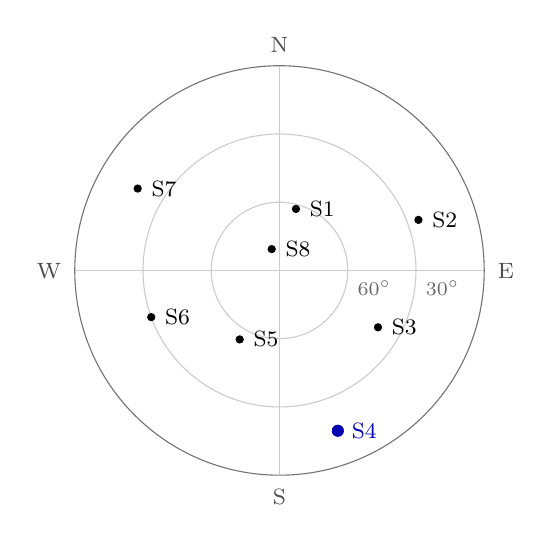
\begin{tikzpicture}
  \def\laR{2.6}
  \draw[black!20] (0,0) circle ({\laR/3});
  \draw[black!20] (0,0) circle ({2*\laR/3});
  \draw[black!55] (0,0) circle (\laR);
  \draw[black!20] (0,-\laR) -- (0,\laR);
  \draw[black!20] (-\laR,0) -- (\laR,0);
  \node[font=\footnotesize, text=black!70, anchor=south] at (0,\laR+0.05) {N};
  \node[font=\footnotesize, text=black!70, anchor=west] at (\laR+0.05,0) {E};
  \node[font=\footnotesize, text=black!70, anchor=north] at (0,-\laR-0.05) {S};
  \node[font=\footnotesize, text=black!70, anchor=east] at (-\laR-0.05,0) {W};
  \node[font=\scriptsize, text=black!60, anchor=north west] at ({\laR/3},0) {$60^\circ$};
  \node[font=\scriptsize, text=black!60, anchor=north west] at ({2*\laR/3},0) {$30^\circ$};
  \foreach \az/\el/\nm in {15/62/S1, 70/25/S2, 120/40/S3, 210/55/S5,
                           250/30/S6, 300/18/S7, 340/80/S8} {
    \fill ({90-\az}:{\laR*(90-\el)/90}) circle (1.5pt)
      node[right=1.5pt, font=\footnotesize] {\nm};
  }
  \fill[blue!70!black] ({90-160}:{\laR*75/90}) circle (2.2pt)
    node[right=1.5pt, font=\footnotesize] {S4};
\end{tikzpicture}
\caption{Sky plot of the eight satellites used in every example: azimuth
clockwise from north, zenith at the centre, horizon at the rim.  S4, at
$15^\circ$ elevation, carries the multipath error of Example~1.  No
satellite is below the horizon, which is the geometric reason for
Example~8.}
\label{fig:la-skyplot}
\end{figure}

\begin{center}
\small
\begin{tabular}{@{}l>{\raggedright\arraybackslash}p{0.66\linewidth}@{}}
\toprule
Setting & Value \\
\midrule
Signal & GPS L1, $\lambda_{\mathrm{L1}} = 0.1903$~m \\
Azimuth / elevation & S1 $15^\circ/62^\circ$, S2 $70^\circ/25^\circ$,
  S3 $120^\circ/40^\circ$, S4 $160^\circ/15^\circ$, S5 $210^\circ/55^\circ$,
  S6 $250^\circ/30^\circ$, S7 $300^\circ/18^\circ$, S8 $340^\circ/80^\circ$ \\
Code $\sigma_\code$ & $0.3$~m (geodetic receiver); $3$~m (low-cost receiver,
  Example~11) \\
Phase $\sigma_\phaseo$ & $3$~mm (geodetic receiver); $2$~mm (low-cost
  receiver) \\
\bottomrule
\end{tabular}
\end{center}

% ------------------------------------------------------------
\subsection{Norms}\label{sec:la-norms}

\paragraph{Four norms and their unit balls.}
\begin{equation}
\lVert\bm{v}\rVert_1 = \sum_i |v_i|,
\qquad
\lVert\bm{v}\rVert_2 = \Bigl(\sum_i v_i^2\Bigr)^{1/2},
\qquad
\lVert\bm{v}\rVert_\infty = \max_i |v_i|,
\qquad
\lVert\bm{v}\rVert_{\bm{W}} = \bigl(\bm{v}^\Tr\bm{W}\,\bm{v}\bigr)^{1/2},
\label{eq:la-norms}
\end{equation}
where $\bm{W}$ is symmetric positive definite.  The first three treat every
component alike.  The fourth builds its metric from a matrix, and in
estimation that matrix is an inverse covariance (\Cref{fig:la-balls}).

\begin{figure}[htbp]
\centering
\begin{tikzpicture}[scale=1.3]
  \draw[black!25] (-2.2,0) -- (2.2,0) node[right, text=black!60, font=\footnotesize] {$x_1$};
  \draw[black!25] (0,-1.35) -- (0,1.35) node[above, text=black!60, font=\footnotesize] {$x_2$};
  \draw[semithick, densely dotted] (-1,-1) rectangle (1,1);
  \draw[semithick] (0,0) circle (1);
  \draw[semithick, dashed] (1,0) -- (0,1) -- (-1,0) -- (0,-1) -- cycle;
  \draw[thick, blue!70!black, rotate=31.72] (0,0) ellipse (1.535 and 0.586);
  \node[anchor=south east, font=\footnotesize] at (-1.02,1.02) {$\lVert\bm{x}\rVert_\infty = 1$};
  \node[anchor=south west, font=\footnotesize] at (1.15,1.02) {$\bm{x}^\Tr\bm{Q}^{-1}\bm{x} = 1$};
  \draw[black!50] (-25:1) -- (1.28,-0.62)
    node[right, font=\footnotesize, text=black] {$\lVert\bm{x}\rVert_2 = 1$};
  \draw[black!50] (0.62,-0.38) -- (1.28,-1.02)
    node[right, font=\footnotesize, text=black] {$\lVert\bm{x}\rVert_1 = 1$};
\end{tikzpicture}
\caption{Unit balls of the four norms of \Cref{eq:la-norms} in the plane:
the L1 diamond (dashed), the L2 circle (solid), the L$\infty$ square
(dotted) and, in blue, the weighted norm with $\bm{W} = \bm{Q}^{-1}$ for
$\bm{Q} = \left[\begin{smallmatrix} 1.8 & 0.9 \\ 0.9 & 0.9
\end{smallmatrix}\right]$.  Its unit ball is an ellipse with axes along the
eigenvectors of $\bm{Q}$ and semi-axes $\sqrt{\lambda_i(\bm{Q})}$; whitening
by the Cholesky factor of $\bm{Q}$ maps it onto the circle.}
\label{fig:la-balls}
\end{figure}

\paragraph{Least squares picks its norm from the covariance.}
Weighted least squares minimises a weighted L2 norm of the residuals,
\begin{equation}
\hat{\bm{x}} = \arg\min_{\bm{x}}\,
  \lVert\bm{y} - \bm{A}\bm{x}\rVert^2_{\Rmat^{-1}},
\label{eq:la-wls-norm}
\end{equation}
so choosing the weight matrix is choosing the norm.  With the Cholesky
factor $\Rmat = \bm{L}\bm{L}^\Tr$, the whitened quantities
$\bar{\bm{y}} = \bm{L}^{-1}\bm{y}$ and $\bar{\bm{A}} = \bm{L}^{-1}\bm{A}$ have
unit covariance, and \Cref{eq:la-wls-norm} becomes ordinary least squares,
$\min\lVert\bar{\bm{y}} - \bar{\bm{A}}\bm{x}\rVert_2^2$.  The same squared
norm returns throughout GNSS quality control:
\begin{itemize}[leftmargin=*, itemsep=1pt]
\item the overall model test behind RAIM,
      $T = \hat{\bm{\varepsilon}}^\Tr\Rmat^{-1}\hat{\bm{\varepsilon}}
      \sim \chi^2(m-n)$ when the model is correct
      (\dcref{sec:stoch-vf}{the variance-factor section of the Stochastic
      Model and QC document});
\item the Kalman innovation test,
      $\innov^\Tr\Smat^{-1}\innov \sim \chi^2(m_k)$
      (\dcref{sec:kf-gating}{the gating section of the Kalman filter
      document});
\item integer least squares,
      $\ambfix = \arg\min_{\bm{a}\in\mathbb{Z}^n}
      \lVert\ambfloat - \bm{a}\rVert^2_{\ambcov^{-1}}$
      (\dcref{eq:ils}{the integer least-squares problem of the Ambiguity
      Resolution document}), whose ratio test compares the two smallest
      values of this norm.
\end{itemize}
The residuals are a projection of the data,
\begin{equation}
\hat{\bm{\varepsilon}} = (\bm{I} - \bm{\Pi}_A)\,\bm{y},
\qquad
\bm{\Pi}_A = \bm{A}\bm{N}^{-1}\bm{A}^\Tr\bm{W}.
\label{eq:la-projector}
\end{equation}
For uncorrelated observations the diagonal entries $r_\sat$ of
$\bm{I} - \bm{\Pi}_A$ are the redundancy numbers of
\dcref{eq:qc-redundancy}{the Stochastic Model and QC document}.  They sum
to $m - n$, and $r_\sat$ is the share of an error in observation $\sat$
that stays visible in its own residual.

\paragraph{L1: bounding the influence of one observation.}
The L2 norm squares residuals, so a single large error dominates the fit.
Least absolute deviations, $\min\lVert\bm{y}-\bm{A}\bm{x}\rVert_1$, grow
only linearly with the residual.  Robust GNSS estimators sit between the two
and run as iteratively reweighted least squares.  The Huber function is
quadratic near zero and linear in the tails,
\begin{equation}
\rho(v) =
\begin{cases}
\tfrac12 v^2, & |v| \le k, \\
k|v| - \tfrac12 k^2, & |v| > k,
\end{cases}
\qquad
w(v) = \min\Bigl(1, \frac{k}{|v|}\Bigr),
\label{eq:la-huber}
\end{equation}
with $v$ the standardised residual and $w$ the weight of the next
iteration.  The IGG-III and Danish schemes go further and drive the weight
of large residuals toward zero.

\paragraph{Example 1 (a multipath error on a low satellite).}
\phantomsection\label{la:ex1}%
S4 ($15^\circ$ elevation) delivers a non-line-of-sight signal with a
$+20$~m range error; the other code errors are Gaussian with
$\sigma = 0.3$~m.  Over 4000 trials:
\begin{center}
\small
\begin{tabular}{@{}lr@{}}
\toprule
Estimator & RMS 3-D position error \\
\midrule
Least squares, no fault & $0.52$~m \\
Least squares, with the fault & $12.89$~m \\
Huber, $k = 1.5$ & $1.15$~m \\
L1 (least absolute deviations) & $0.99$~m \\
Least squares, S4 excluded & $0.61$~m \\
\bottomrule
\end{tabular}
\end{center}
Least squares hides the fault.  The redundancy number of S4 is
$r_4 = 0.354$, so only $7.1$~m of the $20$~m error stays in its own
residual; the rest moves the solution by $(-1.9,\ 7.7,\ 10.2)$~m in east,
north and up and by $8.0$~m in the clock.  The low satellites have the
smallest redundancy numbers (S7 at $18^\circ$: $0.258$; S2 and S4:
$0.354$; S3 at $40^\circ$: $0.673$).  This fault is large enough for
Baarda's $w$-test \cite{baarda1968testing} to flag: the expected statistic
of \dcref{eq:qc-wtest-diag}{the diagonal $w$-test} is
$20\sqrt{r_4}/0.3 = 39.7$ against a critical value of $3.29$.  The minimal
detectable bias of \dcref{eq:qc-mdb}{the MDB formula} for S4 is, however,
$2.1$~m: a smaller multipath error passes the test and still biases the
position.  The robust estimators cut the error by a factor of 11 to 13 with
no explicit detection step, and excluding S4 after detection returns
$0.61$~m.

\paragraph{L$\infty$: rounding, integrity and convergence.}
Rounding each float ambiguity to its nearest integer treats the coordinates
separately.  It returns the integer vector nearest in the unweighted L2
norm, and its pull-in region, the set of float values that round to
$\bm{a}$, is a unit cube, which is a ball of the L$\infty$ norm:
\begin{equation}
\mathcal{R}_{\bm{a}} = \bigl\{\bm{x} :
  \lVert\bm{x}-\bm{a}\rVert_\infty \le \tfrac12\bigr\}.
\label{eq:la-pullin-round}
\end{equation}
Integer least squares measures distance in the $\ambcov^{-1}$ norm instead.
Its pull-in regions are Voronoi cells, hexagons in two dimensions:
\begin{equation}
\mathcal{S}_{\bm{a}} = \bigl\{\bm{x} :
  \lVert\bm{x}-\bm{a}\rVert_{\ambcov^{-1}} \le
  \lVert\bm{x}-\bm{u}\rVert_{\ambcov^{-1}}
  \ \text{for all } \bm{u}\in\mathbb{Z}^n\bigr\}.
\label{eq:la-pullin-ils}
\end{equation}
The L$\infty$ norm has two other everyday roles.  Integrity monitoring
bounds the largest position error over the fault modes it considers, and
iterative solvers stop when $\lVert\Delta\bm{x}\rVert_\infty$ falls below a
tolerance.

\paragraph{Example 2 (rounding versus integer least squares).}
\phantomsection\label{la:ex2}%
Two float ambiguities with standard deviations of $0.30$ and $0.26$ cycles
and a correlation of $0.96$.  Success rates from $10^6$ Monte Carlo
samples:
\begin{center}
\small
\begin{tabular}{@{}lrrrr@{}}
\toprule
Covariance & Correlation & $\kappa$ & Rounding & Integer LS \\
\midrule
$\ambcov$ & $0.96$ & $50.1$ & $0.900$ & $0.957$ \\
$\bm{Q}_{\hat z} = \Zmat\ambcov\Zmat^\Tr$ & $0.03$ & $7.8$ & $0.957$ & $0.957$ \\
\bottomrule
\end{tabular}
\end{center}
The transformation
$\Zmat = \left[\begin{smallmatrix} 1 & -1 \\ 1 & -2 \end{smallmatrix}\right]$
has integer entries and determinant $-1$, so it maps integers to integers
and preserves $\det\ambcov$ ($4.77\times10^{-4}$~cycles$^4$ before and
after).  Integer least squares does not change under it; rounding improves
until it matches (\Cref{fig:la-pullin}).  Rounding also cannot use the
correlation: at correlations of $0.98$ and $0.99$ it stays at $0.903$ and
$0.904$, while integer least squares rises to $0.973$ and $0.989$.  The
decorrelation of \dcref{sec:ar-lambda}{the LAMBDA section of the Ambiguity
Resolution document} makes the search space nearly spherical so that the
integer search is fast \cite{teunissen1995lambda}; it does not change the
answer.

\begin{figure}[htbp]
\centering
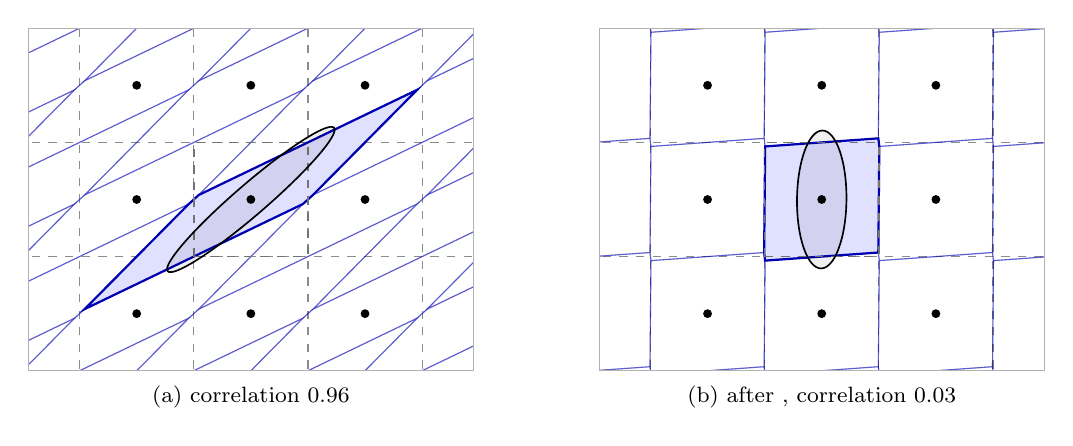
\begin{tikzpicture}[scale=1.45]
  \def\lahexa{(-0.4560,0.0397) -- (-0.5440,-0.0397) -- (-1.4560,-0.9603)
    -- (0.4560,-0.0397) -- (0.5440,0.0397) -- (1.4560,0.9603) -- cycle}
  \def\lahexb{(0.4957,0.5354) -- (-0.4957,0.4646) -- (-0.5043,-0.4646)
    -- (-0.4957,-0.5354) -- (0.4957,-0.4646) -- (0.5043,0.4646) -- cycle}
  % (a) correlated float ambiguities
  \begin{scope}
    \clip (-1.95,-1.5) rectangle (1.95,1.5);
    \draw[black!45, dashed, shift={(0.5,0.5)}] (-3,-3) grid (3,3);
    \foreach \i in {-3,...,3} \foreach \j in {-3,...,3} {
      \draw[blue!70!black, opacity=0.4, shift={(\i,\j)}] \lahexa;
    }
    \filldraw[thick, draw=blue!70!black, fill=blue!12] \lahexa;
    \draw[semithick, black!55, dashed] (-0.5,-0.5) rectangle (0.5,0.5);
    \draw[semithick, fill=black, fill opacity=0.06, rotate=40.75]
      (0,0) ellipse (0.9621 and 0.1360);
    \foreach \i in {-1,0,1} \foreach \j in {-1,0,1} { \fill (\i,\j) circle (1.1pt); }
  \end{scope}
  \draw[black!30] (-1.95,-1.5) rectangle (1.95,1.5);
  \node[font=\footnotesize, anchor=north] at (0,-1.55) {(a) correlation $0.96$};
  % (b) after the Z-transformation
  \begin{scope}[shift={(5.0,0)}]
    \begin{scope}
      \clip (-1.95,-1.5) rectangle (1.95,1.5);
      \draw[black!45, dashed, shift={(0.5,0.5)}] (-3,-3) grid (3,3);
      \foreach \i in {-3,...,3} \foreach \j in {-3,...,3} {
        \draw[blue!70!black, opacity=0.4, shift={(\i,\j)}] \lahexb;
      }
      \filldraw[thick, draw=blue!70!black, fill=blue!12] \lahexb;
      \draw[semithick, black!55, dashed] (-0.5,-0.5) rectangle (0.5,0.5);
      \draw[semithick, fill=black, fill opacity=0.06, rotate=89.40]
        (0,0) ellipse (0.6040 and 0.2166);
      \foreach \i in {-1,0,1} \foreach \j in {-1,0,1} { \fill (\i,\j) circle (1.1pt); }
    \end{scope}
    \draw[black!30] (-1.95,-1.5) rectangle (1.95,1.5);
    \node[font=\footnotesize, anchor=north] at (0,-1.55) {(b) after $\Zmat$, correlation $0.03$};
  \end{scope}
\end{tikzpicture}
\caption{Pull-in regions for the two covariances of Example~2, drawn to
scale in cycles; dots are integer vectors and the correct one is at the
centre.  Dashed grey: rounding cells, the unit squares of
\Cref{eq:la-pullin-round}.  Blue: integer least-squares cells of
\Cref{eq:la-pullin-ils}, the central one shaded.  Grey ellipse: the
$95\,\%$ region of the float solution.  In (a) the float solution reaches
well outside the central square but only to the edge of the central
hexagon.  In (b) the two kinds of cell nearly coincide, which is why
rounding matches integer least squares after decorrelation.}
\label{fig:la-pullin}
\end{figure}

\paragraph{Matrix norms and the condition number.}
\begin{equation}
\lVert\bm{A}\rVert_2 = \sigma_{\max}(\bm{A}),
\qquad
\lVert\bm{A}\rVert_F = \Bigl(\sum_{i,j} a_{ij}^2\Bigr)^{1/2}
  = \Bigl(\sum_i \sigma_i^2\Bigr)^{1/2},
\qquad
\kappa_2(\bm{A}) = \frac{\sigma_{\max}}{\sigma_{\min}}.
\label{eq:la-matnorms}
\end{equation}
The condition number bounds how far relative errors in the data can grow in
the solution.  In floating point a solve loses roughly $\log_{10}\kappa$ of
the 16 significant digits that double precision carries, and forming normal
equations squares it: $\kappa_2(\bm{A}^\Tr\bm{A}) = \kappa_2(\bm{A})^2$
\cite{higham2002accuracy}.

\paragraph{Example 3 (dilution of precision is a matrix norm).}
\phantomsection\label{la:ex3}%
With unit weights, $\covM_{\hat x} = (\bm{G}^\Tr\bm{G})^{-1} =
\bm{V}\bm{\Sigma}^{-2}\bm{V}^\Tr$, so
\begin{equation}
\mathrm{GDOP} = \sqrt{\operatorname{tr}\,(\bm{G}^\Tr\bm{G})^{-1}}
  = \Bigl(\sum_i \sigma_i^{-2}\Bigr)^{1/2}
  = \lVert\bm{G}^{+}\rVert_F .
\label{eq:la-gdop}
\end{equation}
For \Cref{fig:la-skyplot} the singular values of $\bm{G}$ are $3.331$,
$1.668$, $1.331$ and $0.590$, and both sides equal $1.9705$.  The spectral
norm $\lVert\bm{G}^{+}\rVert_2 = 1/\sigma_{\min} = 1.694$ is the largest
gain from a unit-norm vector of range errors to position and clock.  GDOP
averages over all directions; the spectral norm is the worst case.  The
partial measures are HDOP $0.983$, VDOP $1.423$ and TDOP $0.944$.

\paragraph{Example 4 (a determinant does not measure conditioning).}
\phantomsection\label{la:ex4}%
Scaling an $n \times n$ matrix by $c$ gives $\det(c\bm{N}) = c^{\,n}\det\bm{N}$
but leaves $\kappa(c\bm{N}) = \kappa(\bm{N})$.  For the code-only normal
matrix with five parameters (east, north, up, clock, zenith wet delay, the
state of \dcref{sec:estinfra-wls}{the WLS seed of the Estimator
Infrastructure document}) and weights $1/\sigma^2$:
\begin{center}
\small
\begin{tabular}{@{}lrr@{}}
\toprule
$\sigma$ & $\det\bm{N}$ & $\kappa(\bm{N})$ \\
\midrule
$0.3$~m & $2.8\times10^{6}$  & $1.93\times10^{3}$ \\
$1$~m   & $16.4$             & $1.93\times10^{3}$ \\
$3$~m   & $2.8\times10^{-4}$ & $1.93\times10^{3}$ \\
$5$~m   & $1.7\times10^{-6}$ & $1.93\times10^{3}$ \\
\bottomrule
\end{tabular}
\end{center}
A guard that rejects the solution when the determinant falls below a fixed
threshold, such as \dcref{eq:estinfra-wls-detguard}{the determinant guard of
the WLS seed}, responds to the variance units and not to the geometry: the
same satellites pass easily at $0.3$~m and approach the threshold as the
variances grow.  A scale-invariant rank test compares each singular value
with the largest (for a symmetric positive semidefinite matrix, the
eigenvalues) and counts those below $\tau\,\sigma_{\max}$.  The table also
prices the zenith delay: $\kappa(\bm{G}^\Tr\bm{G})$ is $31.8$ for position
and clock alone and $1933$ once the delay joins them, because its mapping
function (roughly $1/\sin e$) is one more function of elevation that the up
and clock columns nearly reproduce.

% ------------------------------------------------------------
\subsection{Hermitian matrices}\label{sec:la-hermitian}

A matrix is Hermitian when it equals its conjugate transpose,
$\bm{A} = \bm{A}^{\mathsf{H}}$.  For real matrices that is symmetry, and
every covariance, weight, normal and Kalman covariance matrix in GNSS
estimation is real symmetric.  The spectral theorem gives
\begin{equation}
\bm{Q} = \bm{V}\bm{\Lambda}\bm{V}^\Tr,
\qquad
\bm{V}^\Tr\bm{V} = \bm{I},
\qquad
\lambda_i \in \mathbb{R},
\label{eq:la-spectral}
\end{equation}
and a covariance matrix is positive semidefinite, $\lambda_i \ge 0$.  The
eigenvalues bound the variance in any direction $\bm{d}$ (the Rayleigh
quotient):
\begin{equation}
\lambda_{\min} \le
  \frac{\bm{d}^\Tr\bm{Q}\,\bm{d}}{\bm{d}^\Tr\bm{d}}
  \le \lambda_{\max}.
\label{eq:la-rayleigh}
\end{equation}
Complex Hermitian matrices appear one level down, in the receiver's signal
processing (Example~7).

\paragraph{Example 5 (an error ellipse is an eigendecomposition).}
\phantomsection\label{la:ex5}%
Code-only solution for \Cref{fig:la-skyplot} with $\sigma = 0.3$~m.  The
horizontal block of $\covM_{\hat x} = \sigma^2(\bm{G}^\Tr\bm{G})^{-1}$ is
\begin{equation*}
\bm{Q}_{EN} = \begin{bmatrix} 0.0337 & 0.0053 \\ 0.0053 & 0.0533 \end{bmatrix}\ \mathrm{m}^2 .
\end{equation*}
Its eigenvalues, $0.0547$ and $0.0324$~m$^2$, give $1\sigma$ semi-axes of
$0.234$ and $0.180$~m.  A $95\,\%$ region in two dimensions scales them by
$\sqrt{\chi^2_{2}(0.95)} = 2.448$, to $0.572$ by $0.440$~m, with the major
axis along the first eigenvector at azimuth $14.1^\circ$.  The vertical
standard deviation is larger, $0.427$~m, for the reason Example~8 gives.

\paragraph{Cholesky: whitening, simulation, decorrelation.}
A symmetric positive definite matrix factors as $\bm{Q} = \bm{L}\bm{L}^\Tr$
with $\bm{L}$ lower triangular.  The factor is used for
\begin{itemize}[leftmargin=*, itemsep=1pt]
\item solving the normal equations, at half the cost of an LU factorisation
      and without pivoting;
\item whitening correlated observations: $\bm{L}^{-1}\bm{y}$ has identity
      covariance (the network producer whitens its correlated
      pseudo-observation blocks this way, \dcref{sec:atmos-shvtec}{the
      spherical-harmonic VTEC section of the Atmosphere document});
\item simulating correlated noise: $\bm{\varepsilon} = \bm{L}\bm{z}$ with
      $\bm{z}\sim N(\bm{0},\bm{I})$;
\item in the form $\ambcov = \Lmat^\Tr\Dmat\Lmat$, the LAMBDA decorrelation
      and search (\dcref{eq:ldlt}{the $\mathrm{LDL}^\Tr$ factorisation of the
      Ambiguity Resolution document}).
\end{itemize}

\paragraph{Example 6 (double differences share a reference satellite).}
\phantomsection\label{la:ex6}%
With undifferenced variance $\sigma^2$ on every phase observation, $n$
double differences (\dcref{sec:dd}{the double-difference section of the
Foundations document}) against one reference satellite have
\begin{equation}
\bm{Q}_{\dd{}} = 2\sigma^2\bigl(\bm{I}_n + \bm{1}\bm{1}^\Tr\bigr),
\qquad
\bm{Q}_{\dd{}}^{-1} = \frac{1}{2\sigma^2}
  \Bigl(\bm{I}_n - \frac{\bm{1}\bm{1}^\Tr}{n+1}\Bigr),
\label{eq:la-ddcov}
\end{equation}
the inverse following from the Sherman--Morrison formula.  The eigenvalues
are $2\sigma^2$ with multiplicity $n-1$ and $2\sigma^2(n+1)$ along
$\bm{1}$.  For eight satellites ($n = 7$) and $\sigma = 3$~mm they are
$18$~mm$^2$ six times and $144$~mm$^2$ once.  The reference satellite's
error enters every double difference, so the common-mode direction carries
eight times the variance of any other.  Treating the double differences as
independent, each with its true variance $4\sigma^2$, overweights that
common mode by a factor of 4 and underweights every other direction by a
factor of 2.  The inverse above, or whitening by the Cholesky factor,
weights them correctly.

\paragraph{Example 7 (antenna arrays: a complex Hermitian covariance).}
\phantomsection\label{la:ex7}%
An array of $M$ elements sampling complex baseband (I/Q) snapshots
$\bm{s}(t) \in \mathbb{C}^M$ has the spatial covariance
\begin{equation}
\bm{C}_s = \mathsf{E}\{\bm{s}\,\bm{s}^{\mathsf{H}}\}
  = \sum_k p_k\,\bm{\alpha}(\theta_k)\,\bm{\alpha}(\theta_k)^{\mathsf{H}}
  + \sigma_n^2\bm{I},
\label{eq:la-array}
\end{equation}
which is Hermitian and positive definite; $\bm{\alpha}(\theta)$ is the
steering vector of a source at angle $\theta$ and $p_k$ its power.  GNSS
signals arrive 20 to 30~dB below the thermal noise, so the eigenvectors with
large eigenvalues belong to interference.  Projecting onto their orthogonal
complement,
$\bm{\Pi}^{\perp} = \bm{I} - \bm{U}_J\bm{U}_J^{\mathsf{H}}$,
removes the interference without knowing where the satellites are
\cite{kaplan2017understanding}.  With four elements at half-wavelength
spacing, a jammer at $40^\circ$ with a jammer-to-noise ratio of $40$~dB, a
satellite at $-15^\circ$ with a signal-to-noise ratio of $-20$~dB, and 4000
snapshots:
\begin{itemize}[leftmargin=*, itemsep=1pt]
\item the sample covariance has eigenvalues $0.98$, $1.00$, $1.03$ and
      $39\,648$ (noise power 1).  One stands out, near $M$ times the jammer
      power; the satellite does not show in the spectrum at all;
\item the projection attenuates the jammer direction by $77.9$~dB and costs
      the satellite direction $0.09$~dB.
\end{itemize}
\begin{center}
\small
\begin{tabular}{@{}lr@{}}
\toprule
Array weights & Output signal-to-jammer-plus-noise ratio \\
\midrule
Single element & $-60.0$~dB \\
Beam steered at the satellite & $-43.3$~dB \\
Projection, then beam & $-14.1$~dB \\
MVDR, $\bm{w} \propto \bm{C}_s^{-1}\bm{\alpha}(\theta_{\mathrm{sat}})$ & $-14.1$~dB \\
\bottomrule
\end{tabular}
\end{center}
The last two recover the full array gain of a clean sky,
$-20~\mathrm{dB} + 10\log_{10}4 = -14.0$~dB.  Correlation with the spreading
code then lifts the signal above the noise as usual.

\paragraph{Keeping a Kalman covariance symmetric and positive definite.}
Rounding error erodes symmetry and positive definiteness in the short-form
update $(\bm{I} - \Kgain\jacH)\covM$, most of all when states with
millimetre-level uncertainty (converged ambiguities) share the matrix with
states whose uncertainty is kilometres (a freshly initialised clock).  The
engine uses the Joseph form and symmetrises the result
(\dcref{eq:kf-joseph}{the Joseph-form update of the Kalman filter
document}).  Square-root and UD filters go further: they carry a factor
$\bm{S}$ with $\covM = \bm{S}\bm{S}^\Tr$ and
$\kappa(\bm{S}) = \sqrt{\kappa(\covM)}$ \cite{bierman1977factorization}.
These, and not the pseudoinverse, are the tools for a filter whose code and
phase precisions differ by three orders of magnitude.

% ------------------------------------------------------------
\subsection{The singular value decomposition}\label{sec:la-svd}

Every real $m \times n$ matrix factors as
\begin{equation}
\bm{A} = \bm{U}\bm{\Sigma}\bm{V}^\Tr = \sum_{i=1}^{r}\sigma_i\,\bm{u}_i\bm{v}_i^\Tr,
\qquad
\sigma_1 \ge \sigma_2 \ge \dots \ge \sigma_r > 0,
\label{eq:la-svd}
\end{equation}
with orthonormal $\bm{u}_i$ in observation space and $\bm{v}_i$ in
parameter space.  A parameter change along $\bm{v}_i$ moves the
observations by $\sigma_i$ along $\bm{u}_i$.  The $\sigma_i^2$ are the
eigenvalues of $\bm{A}^\Tr\bm{A}$, and for a symmetric positive
semidefinite matrix the eigenvalues and singular values coincide.  The
numerical rank is the number of $\sigma_i$ above a tolerance $\tau\sigma_1$.
The $\bm{v}_i$ with $\sigma_i \approx 0$ span the null space: parameter
combinations the data cannot see.  In a network that estimates every
receiver and satellite clock, adding one constant to all of them leaves
every observation unchanged, so a zero singular value is structural there
(Example~13; \dcref{sec:net-example}{the two-receiver worked example of the
Network-mode document}).  The network producer counts such directions from
the eigenvalues of its reduced normals before every solve
(\dcref{sec:net-sbasis}{the S-basis section of the Network-mode document}).

\paragraph{Example 8 (the weakest direction of the geometry).}
\phantomsection\label{la:ex8}%
The right singular vector for the smallest singular value of $\bm{G}$
($0.590$) is
\begin{equation*}
\bm{v}_4 = (-0.03,\ -0.14,\ 0.83,\ 0.54)
\quad\text{in (east, north, up, clock).}
\end{equation*}
Raising the antenna by $0.83$~m while advancing the clock by $0.54$~m
changes the eight ranges by $0.32$~m at most.  The clock column is all ones
and the up column is $-\sin e_\sat$, negative for every satellite above the
horizon, so the two columns are close to parallel: the up and clock
estimates correlate at $+0.93$, and VDOP ($1.42$) exceeds HDOP ($0.98$).
Satellites below the horizon would break the near-parallelism, which is why
ground-based GNSS measures height worse than horizontal position.

\paragraph{Example 9 (attitude from antenna baselines).}
\phantomsection\label{la:ex9}%
Three antennas on a vehicle give two baselines with known body-frame
vectors $\bm{b}_k$ ($1.5$~m forward and $1.0$~m to the side) and
RTK-measured local-frame vectors $\bm{r}_k$.  The attitude is the
rotation that minimises $\sum_k \lVert\bm{r}_k - \bm{C}\bm{b}_k\rVert^2$
(Wahba's problem \cite{wahba1965least}).  With
$\bm{B} = \sum_k \bm{r}_k\bm{b}_k^\Tr = \bm{U}\bm{\Sigma}\bm{V}^\Tr$
\cite{markley1988attitude},
\begin{equation}
\hat{\bm{C}} = \bm{U}\,\operatorname{diag}\bigl(1,\ 1,\
  \det(\bm{U}\bm{V}^\Tr)\bigr)\,\bm{V}^\Tr .
\label{eq:la-wahba}
\end{equation}
An unconstrained $3 \times 3$ fit would have nine unknowns and six
equations; the rotation constraint makes the problem well posed, and the
SVD solves it in closed form.  With $3$~mm noise on each baseline component
over 5000 trials, the RMS errors are $0.095^\circ$ in yaw, $0.116^\circ$ in
pitch and $0.171^\circ$ in roll.  Each error follows its baseline: roll
depends on the $1.0$~m side baseline ($3$~mm over $1.0$~m is $0.17^\circ$)
and pitch on the $1.5$~m forward one ($0.11^\circ$).  $\bm{B}$ has rank 2
(singular values $2.25$, $0.99$ and $0$), and the determinant term fixes
the third axis.

The same step keeps an inertial attitude matrix orthonormal.  Replacing a
drifted attitude matrix $\bm{C}$ (the $\Cbe$ of the inertial path) by
$\bm{U}\bm{V}^\Tr$ from its SVD gives the nearest orthogonal matrix in the
Frobenius norm: in the example
$\lVert\bm{C}^\Tr\bm{C} - \bm{I}\rVert_F$ drops from $5.2\times10^{-3}$ to
$9\times10^{-16}$.  The engine applies it during strapdown integration and
after every attitude feedback (\dcref{sec:imu-mech}{the strapdown section
of the Inertial Aiding document}).

\paragraph{Example 10 (common-mode error in a regional network).}
\phantomsection\label{la:ex10}%
Daily coordinate residuals of the stations in a regional network share a
common-mode signal from reference-frame, large-scale atmospheric and
loading errors.  With the residual matrix $\bm{X}$ (days $\times$ stations,
column means removed), the leading term $\sigma_1\bm{u}_1\bm{v}_1^\Tr$ of its
SVD estimates that signal: $\bm{u}_1$ carries its time series and
$\bm{v}_1$ each station's response \cite{dong2006spatiotemporal}.  The
example is synthetic: up component, 12 stations, 730 days, a
time-correlated common signal of $2.5$~mm scaled by a station response
between $0.8$ and $1.2$, and $2.0$~mm of white noise per station.
\begin{itemize}[leftmargin=*, itemsep=1pt]
\item The first component carries $66.1\,\%$ of the variance; the next two,
      $3.9\,\%$ and $3.6\,\%$.
\item Removing it lowers the mean station RMS from $3.27$~mm to $1.91$~mm,
      the white-noise level.
\item The recovered series correlates $0.977$ with the true common mode, and
      $\bm{v}_1$ correlates $0.962$ with the true station responses.
\end{itemize}

\paragraph{Ill-posed inversions: truncated SVD and Tikhonov.}
Ionospheric and water-vapour tomography lead to systems whose singular
values decay toward zero with no clear gap.  The least-squares solution
\begin{equation}
\hat{\bm{x}} = \sum_i \frac{\bm{u}_i^\Tr\bm{y}}{\sigma_i}\,\bm{v}_i
\label{eq:la-svd-solution}
\end{equation}
then amplifies noise through the small $\sigma_i$.  Truncated SVD keeps the
first $k$ terms; Tikhonov regularisation replaces $1/\sigma_i$ by
$\sigma_i/(\sigma_i^2 + \alpha^2)$.  Both accept bias to reduce variance,
with $k$ or $\alpha$ chosen from the data (the L-curve, generalised
cross-validation).  That is a deliberate choice for an ill-posed problem,
and a different thing from what a default pseudoinverse tolerance does to a
well-posed one (Example~11).  The engine's SP3 orbit fit solves a
well-posed least-squares problem through \Cref{eq:la-svd-solution} with a
relative cutoff (\dcref{sec:prod-trig}{the sidereal-trigonometric fit of
the Orbit and Clock Product Evaluation document}).

% ------------------------------------------------------------
\subsection{The pseudoinverse}\label{sec:la-pinv}

The Moore--Penrose pseudoinverse is $\bm{A}^{+} = \bm{V}\bm{\Sigma}^{+}\bm{U}^\Tr$,
where $\bm{\Sigma}^{+}$ inverts the nonzero singular values and keeps the
zeros.  It is the unique matrix that satisfies the four Penrose conditions
\begin{equation}
\bm{A}\bm{A}^{+}\bm{A} = \bm{A},
\qquad
\bm{A}^{+}\bm{A}\bm{A}^{+} = \bm{A}^{+},
\qquad
(\bm{A}\bm{A}^{+})^\Tr = \bm{A}\bm{A}^{+},
\qquad
(\bm{A}^{+}\bm{A})^\Tr = \bm{A}^{+}\bm{A}.
\label{eq:la-penrose}
\end{equation}
Three cases matter in GNSS.
\begin{itemize}[leftmargin=*, itemsep=1pt]
\item \emph{Full column rank}, as in ordinary positioning:
      $\bm{A}^{+} = (\bm{A}^\Tr\bm{A})^{-1}\bm{A}^\Tr$, so the pseudoinverse is
      least squares computed through the SVD.  With weights,
      $\hat{\bm{x}} = (\bm{W}^{1/2}\bm{A})^{+}\,\bm{W}^{1/2}\bm{y}$; applying
      $\bm{A}^{+}$ to $\bm{y}$ directly drops the weights.
\item \emph{Rank deficient}, as with a datum defect: $\bm{A}^{+}\bm{y}$ is the
      least-squares solution of minimum norm.  It is orthogonal to the null
      space, which means it chooses a datum without saying so (Example~13;
      \cite{teunissen1985generalised}).
\item \emph{Numerically rank deficient}: singular values below $\tau\sigma_1$
      count as zero.  Deliberate truncation regularises an ill-posed problem
      (\Cref{sec:la-svd}); a default tolerance applied to a badly scaled but
      well-posed problem discards real information (Example~11).
\end{itemize}
In the engine the pseudoinverse appears in two full-rank roles: the SP3
orbit fit above, and the fallback of the Kalman gain solve when the
$\mathrm{LDL}^\Tr$ factorisation of $\Smat$ fails (\dcref{sec:kf-update}{the
measurement-update section of the Kalman filter document}).

\paragraph{Example 11 (metre-level code, millimetre-level phase).}
\phantomsection\label{la:ex11}%
One epoch of code and phase, \Cref{eq:la-single-epoch}, with float
ambiguities estimated as corrections to a priori values and a position
offset of $(3,\,-2,\,5)$~m.  The phase-to-code weight ratio is
$(\sigma_\code/\sigma_\phaseo)^2$: $10^4$ for the geodetic receiver and
$2.25\times10^6$ for the low-cost one.  Each solver column gives the
position error against a stable reference, SVD least squares on the
whitened system in double precision.
\begin{center}
\footnotesize
\setlength{\tabcolsep}{4pt}
\begin{tabular}{@{}lrrrrrr@{}}
\toprule
& & & \multicolumn{2}{c}{double precision} & \multicolumn{2}{c}{single precision} \\
\cmidrule(lr){4-5}\cmidrule(l){6-7}
Case & $\kappa(\bm{W}^{1/2}\bm{A})$ & $\kappa(\bm{N})$ & Cholesky on $\bm{N}$
  & $\bm{N}^{+}$ & normal eqs. & QR on $\bm{W}^{1/2}\bm{A}$ \\
\midrule
Geodetic & $1.8\times10^{3}$ & $3.4\times10^{6}$ & $<1$\,\si{\micro\metre} & $<1$\,\si{\micro\metre} & $8.3$~cm & \SI{7}{\micro\metre} \\
Low-cost & $2.8\times10^{4}$ & $7.6\times10^{8}$ & $<1$\,\si{\micro\metre} & $<1$\,\si{\micro\metre} & $\mathbf{42}$~\textbf{m} & \SI{3}{\micro\metre} \\
Clock in seconds & $4.6\times10^{11}$ & $2.1\times10^{23}$ & $<1$\,\si{\micro\metre} & $\mathbf{5.1}$~\textbf{m} & $6.9$~cm & \SI{2}{\micro\metre} \\
\bottomrule
\end{tabular}
\end{center}
\begin{itemize}[leftmargin=*, itemsep=1pt]
\item \emph{Not near-singular.}  Double precision carries about 16 digits,
      and $\kappa(\bm{N})$ between $10^6$ and $10^9$ leaves 7 to 10 of them.
      The weight matrix is diagonal, so its inverse is exact however wide
      its range.
\item \emph{The weight range costs digits through the normal equations},
      because $\kappa(\bm{N}) = \kappa(\bm{W}^{1/2}\bm{A})^2$.  In single
      precision that is the difference between $42$~m and \SI{3}{\micro\metre} in the
      low-cost case.  QR on the whitened system never forms $\bm{N}$.
\item \emph{Units, not information.}  A clock parameter in seconds
      multiplies its column by $\sLight = 2.998\times10^8$~m/s and drives
      $\kappa(\bm{N})$ to $2.1\times10^{23}$.  Cholesky is insensitive to
      this kind of diagonal scaling and still returns the position within
      \SI{1}{\micro\metre}.  The pseudoinverse of $\bm{N}$ with numpy's default relative
      tolerance ($10^{-15}\sigma_1$) sets 11 of its 12 singular values to
      zero and returns the a priori position unchanged: a $5.1$~m error with
      no warning.
\end{itemize}
The remedies are consistent units (the clock in metres, unknowns as
corrections to a priori values), whitening followed by QR or by Cholesky in
double precision, and square-root forms in filters.  The pseudoinverse is
not a remedy for ill-conditioning.

\paragraph{Example 12 (what phase adds to a single epoch).}
\phantomsection\label{la:ex12}%
Order the parameters of \Cref{eq:la-single-epoch} as the position and clock
$\bm{x}$ followed by the ambiguities $N_1,\dots,N_m$, with
$\bm{W}_\code = \sigma_\code^{-2}\bm{I}$ and
$\bm{W}_\phaseo = \sigma_\phaseo^{-2}\bm{I}$.  The normal matrix is
\begin{equation}
\bm{N} =
\begin{bmatrix}
\bm{N}_{xx} & \bm{N}_{xa} \\ \bm{N}_{ax} & \bm{N}_{aa}
\end{bmatrix}
=
\begin{bmatrix}
\bm{G}^\Tr(\bm{W}_\code + \bm{W}_\phaseo)\,\bm{G}
  & \lambda_{\mathrm{L1}}\,\bm{G}^\Tr\bm{W}_\phaseo \\
\lambda_{\mathrm{L1}}\,\bm{W}_\phaseo\bm{G} & \lambda_{\mathrm{L1}}^2\,\bm{W}_\phaseo
\end{bmatrix}.
\label{eq:la-partition}
\end{equation}
Eliminating the ambiguities (the Schur complement) leaves
\begin{equation}
\bm{N}_{xx} - \bm{N}_{xa}\bm{N}_{aa}^{-1}\bm{N}_{ax} = \bm{G}^\Tr\bm{W}_\code\,\bm{G},
\label{eq:la-schur}
\end{equation}
the code-only normal matrix.  With float ambiguities, one epoch of phase
adds nothing to the position: in Example~11 the code-plus-phase and
code-only positions agree to $3\times10^{-13}$~m.  This is the
single-receiver case of the statement in \dcref{sec:stoch-baarda}{the
redundancy section of the Stochastic Model and QC document} that per-arc
float ambiguities leave no phase-side redundancy.  Phase precision reaches
the position only once the ambiguities are fixed to integers or tied
together over time.

The weight range reappears in the float ambiguities:
\begin{equation}
\ambcov = \frac{1}{\lambda_{\mathrm{L1}}^2}
  \Bigl(\sigma_\phaseo^2\,\bm{I}_m + \sigma_\code^2\,\bm{\Pi}_G\Bigr),
\qquad
\bm{\Pi}_G = \bm{G}(\bm{G}^\Tr\bm{G})^{-1}\bm{G}^\Tr .
\label{eq:la-qa}
\end{equation}
$\bm{\Pi}_G$ is an orthogonal projector of rank 4, so the eigenvalues of
$\ambcov$ are $(\sigma_\code^2 + \sigma_\phaseo^2)/\lambda_{\mathrm{L1}}^2$
four times and $\sigma_\phaseo^2/\lambda_{\mathrm{L1}}^2$ the remaining
$m-4$ times, and
\begin{empheq}[box=\fbox]{equation}
\kappa(\ambcov) = 1 + \frac{\sigma_\code^2}{\sigma_\phaseo^2}.
\label{eq:la-kappa-qa}
\end{empheq}
Computed: eigenvalues of $2.486$ and $2.49\times10^{-4}$~cycles$^2$ and
$\kappa = 1.0001\times10^4$ in the geodetic case, and
$\kappa = 2.25\times10^6$ in the low-cost case, both matching
\Cref{eq:la-kappa-qa}.  The ambiguity search space is an ellipsoid 100
times longer than it is wide in the geodetic case and 1500 times in the
low-cost case.  That elongation is why LAMBDA decorrelates before it
searches (Example~2).

\paragraph{Example 13 (a network with a datum defect).}
\phantomsection\label{la:ex13}%
Three receivers track eight satellites, and the only parameters are clocks:
$y_{\rx\sat} = \mathrm{d}t_\rx - \mathrm{d}t^\sat + \varepsilon_{\rx\sat}$ in
metres, with $\sigma = 1$~cm.  Adding the same constant to every clock
leaves every observation unchanged, so $\bm{A}\bm{1} = \bm{0}$: rank 10 for
11 parameters, with a smallest singular value of $3\times10^{-16}$.  This
is the null vector of \dcref{sec:net-example}{the two-receiver worked
example of the Network-mode document}, which compares two pinned datums.
Here the pseudoinverse is the second solution:
\begin{itemize}[leftmargin=*, itemsep=1pt]
\item \emph{Pseudoinverse}: minimum norm, hence
      $\bm{1}^\Tr\hat{\bm{x}}^{+} = 0$; the datum is that the eleven clocks
      sum to zero.
\item \emph{Explicit S-basis}: the first receiver's clock is fixed to zero
      (the pivot) and the remaining full-rank system is solved.
\end{itemize}
\begin{center}
\small
\begin{tabular}{@{}>{\raggedright\arraybackslash}p{0.36\linewidth}>{\raggedright\arraybackslash}p{0.32\linewidth}>{\raggedright\arraybackslash}p{0.24\linewidth}@{}}
\toprule
Quantity & Pseudoinverse & Pivot \\
\midrule
Satellite clock differences $\mathrm{d}t^\sat - \mathrm{d}t^1$ (estimable)
  & \multicolumn{2}{>{\raggedright\arraybackslash}p{0.56\linewidth}}{agree to $2\times10^{-10}$~m} \\
Receiver clocks (not estimable) & $23.6$, $-128.1$, $51.7$~km
  & $0$, $-151.7$, $28.1$~km \\
Trace of the covariance (unit variance) & $2.674$ & $3.833$ \\
Change in the receiver clocks when the $+468$\,\si{\micro\second} satellite sets
  & $+13\,534.8$~m (\SI{45.15}{\micro\second}), all three & $0$, $0.8$, $-7.7$~mm \\
\bottomrule
\end{tabular}
\end{center}
The pseudoinverse has the smaller trace, the minimum-trace property of
free-network adjustment, but it does not remove the defect.  It picks a
datum, and that datum moves whenever the parameter set changes.  For a
departing parameter $x_k$ the jump is $(x_k - \bar{x})/(n-1)$, with
$\bar{x}$ the mean of the $n$ parameters before it left: here
$(468.0 - 16.5)/10 = 45.15$\,\si{\micro\second}, as computed.  GNSS networks
and PPP-RTK therefore choose the S-basis explicitly: a pivot receiver, a
pivot satellite, or a zero-mean condition with rules for set changes
\cite{odijk2016estimability}.  Each estimable combination then has a stated
meaning (\dcref{sec:net-sbasis}{the S-basis section of the Network-mode
document}).

\paragraph{Choosing a solver.}
\begin{center}
\small
\begin{tabular}{@{}>{\raggedright\arraybackslash}p{0.36\linewidth}>{\raggedright\arraybackslash}p{0.58\linewidth}@{}}
\toprule
Situation & Tool \\
\midrule
Full rank, well scaled & Cholesky on $\bm{N}$ in double precision, or QR on
  $\bm{W}^{1/2}\bm{A}$ \\
Wide weight range, single precision, long filters & Whitening and QR; a
  square-root or UD filter for sequential updates \\
Mixed units (seconds, absolute coordinates) & Rescaling: the clock in
  metres, unknowns as corrections to a priori values \\
Datum defect & An explicit S-basis; the pseudoinverse only when estimable
  functions are all that matter \\
Ill-posed inversion (tomography) & Truncated SVD or Tikhonov with a
  data-driven parameter \\
Rank diagnosis & Singular values or eigenvalues relative to the largest,
  never the determinant \\
\bottomrule
\end{tabular}
\end{center}

% ------------------------------------------------------------
\subsection{Exercises}\label{sec:la-exercises}

\begin{enumerate}[leftmargin=*, itemsep=2pt]
\item Show that $\mathrm{GDOP} = \lVert\bm{G}^{+}\rVert_F$ and
      $\lVert\bm{G}^{+}\rVert_2 = 1/\sigma_{\min}$ for a geometry matrix of
      full column rank (\hyperref[la:ex3]{Example~3}).  Which of the two
      answers a worst-case question?
\item Form the partitioned normal matrix \Cref{eq:la-partition}, eliminate
      the ambiguities, and show that the reduced normal matrix equals
      $\bm{G}^\Tr\bm{W}_\code\bm{G}$ (\hyperref[la:ex12]{Example~12}).
      Explain what changes once the ambiguities are fixed to integers.
\item Derive \Cref{eq:la-qa} and the eigenvalues of $\ambcov$, and show
      \Cref{eq:la-kappa-qa}.
\item For $\bm{Q}_{\dd{}}$ of \Cref{eq:la-ddcov}, find the eigenvalues and
      eigenvectors and verify the Sherman--Morrison inverse
      (\hyperref[la:ex6]{Example~6}).  Whiten simulated double differences
      with the Cholesky factor and check that their sample covariance is
      close to the identity.
\item Show that the pseudoinverse solution of \hyperref[la:ex13]{Example~13}
      satisfies $\bm{1}^\Tr\hat{\bm{x}}^{+} = 0$, and derive the jump
      $(x_k - \bar{x})/(n-1)$ when parameter $k$ leaves.
\item In the third case of \hyperref[la:ex11]{Example~11} the clock column
      is scaled by $\sLight$.  Show that column scaling changes $\kappa$ but
      not the least-squares position, then explain why the pseudoinverse of
      $\bm{N}$ failed while Cholesky did not.  (The pseudoinverse tolerance
      is relative to $\sigma_1$.)
\item The WLS seed rejects a solution through the determinant guard of
      \dcref{eq:estinfra-wls-detguard}{the Estimator Infrastructure
      document} (\texttt{WlsEstimator::estimate}).  Use
      \hyperref[la:ex4]{Example~4} to explain what this test measures, and
      replace it with a scale-invariant test.
\item Show that maximising $\operatorname{tr}(\bm{C}^\Tr\bm{B})$ over
      rotations gives \Cref{eq:la-wahba}, and explain why two baselines
      suffice although $\bm{B}$ has rank 2 (\hyperref[la:ex9]{Example~9}).
\item Move the multipath error of \hyperref[la:ex1]{Example~1} from S4 to
      S7.  Predict the change from the redundancy numbers, then run the
      script to check.
\end{enumerate}

% ------------------------------------------------------------
\subsection{Reproducing the numbers and further reading}\label{sec:la-reproduce}

Every number in Examples~1 to 13 is printed by
\begin{center}
\texttt{python scripts/linalg\_supplement\_examples.py}
\end{center}
which needs only numpy and runs in under a minute.  Each example has its
own random seed, so the output is reproducible and one example can be
changed without disturbing the others.

The same operations appear in the engine as follows.
\begin{center}
\small
\begin{tabular}{@{}>{\raggedright\arraybackslash}p{0.42\linewidth}>{\raggedright\arraybackslash}p{0.52\linewidth}@{}}
\toprule
Operation & Symbol (file) \\
\midrule
Cholesky whitening of correlated row blocks into unit-information rows
  & \texttt{Application::networkAppendShIonoRows\_} and its siblings for the GIM
    and single-difference extra-wide-lane rows
    (\texttt{src/core/app/ApplicationNetworkAssembly.cpp}) \\
Condition number of the WLS normal matrix (logged through an SVD) and the
  determinant guard & \texttt{WlsEstimator::estimate}
    (\texttt{src/core/math/WlsEstimator.cpp}) \\
$\mathrm{LDL}^\Tr$ solve of $\Smat$ with a pseudoinverse fallback; Joseph
  update; SVD re-orthonormalisation after attitude feedback
  & \texttt{KalmanFilter::update} (\texttt{src/core/filter/KalmanFilter.cpp}) \\
SVD re-orthonormalisation during strapdown integration
  & \texttt{ImuIntegrator::integrate} (\texttt{src/core/filter/ImuIntegrator.cpp}) \\
SP3 orbit fit by truncated-SVD least squares
  & \texttt{Interpolate::trigSvdInterp} (\texttt{src/core/math/Interpolate.cpp}) \\
Null-space (datum) count from eigenvalues
  & \texttt{NetworkSbasis::assertNullSpaceRank} (\texttt{src/core/filter/NetworkSbasis.cpp}) \\
$\mathrm{LDL}^\Tr$ decorrelation and integer search (MLAMBDA)
  & \texttt{src/core/filter/IlsCore.cpp},
    \texttt{AmbiguityResolver} (\texttt{src/core/filter/AmbiguityResolver.cpp}) \\
\bottomrule
\end{tabular}
\end{center}

For further reading, \textcite{strang2019linear} covers norms, the SVD and the
pseudoinverse at the level of the course; \textcite{higham2002accuracy}
covers conditioning, normal equations against QR, and scaling;
\textcite{teunissen2000adjustment} treats weighted least squares, redundancy
and S-bases in geodetic notation; and \textcite{odijk2016estimability} apply
S-system theory to undifferenced PPP-RTK networks.

\ifSubfilesClassLoaded{\printbibliography}{}
\end{document}
